\documentclass[
    corpo=12pt,
    oneside,
    evenboxes,
    tipotesi=triennale,
    stile=classica,
    oldstyle,
    autoretitolo,
    greek,
]{toptesi}
\usepackage[utf8]{inputenc}
\usepackage[T1]{fontenc}
\usepackage{lmodern}
\usepackage{hyperref}
\usepackage{setspace}
\usepackage{verbatim}
\usepackage{pgfplots}
\usepackage{graphicx}
\usepackage{subfig}
\onehalfspacing

\hypersetup{
    pdfpagemode={UseOutlines},
    bookmarksopen,
    pdfstartview={FitH},
    colorlinks,
    linkcolor={blue},
    citecolor={blue},
    urlcolor={blue}
  }
\usepackage{lipsum}

\newtheorem{osservazione}{Osservazione}

\begin{document}\errorcontextlines=9

\begin{ThesisTitlePage}
    \ateneo{Universit\`a degli Studi di Torino}
    \StrutturaDi{Dipartimento di Management}
    \struttura[]{}
    \NomeElaborato{Tesi di laurea triennale}
    \titolo{Fair Play Fiananziario e Superlega}
    \sottotitolo{Lo stato di salute del Calcio pre e post COVID-19}     
    \corsodistudi{Management dell'Informazione e della Comunicazione Aziendale}
    \candidato{Riccardo \textsc{Borgo}}
    \relatore{prof.ssa ~Simona \textsc{Alfiero}}
    \sedutadilaurea{\textsc{Anno~accademico} 2021-2022}
    \logosede{img/Unito-logo, img/logo_saa.jpeg}
\end{ThesisTitlePage}

\figurespagetrue
\indici

\mainmatter
\begin{interlinea}{1.5}
    
\chapter{Introduzione generale}
Durante lo sviluppo di questa trattazione si andrà ad analizzare l'attuale "stato di salute"
del calcio europeo, di come il \emph{Financial Fair Play} abbia provato da una parte ad aiutare le società a rimanere in regola con i conti e 
dall'altra a dettare delle regole atte ad evitare comportamenti illegali da parte sopratutto dei presidenti.\\
Infine si tratterà il caso della \emph{Superlega}, per cercare di capire se questa nuova idea sia effettivamente coerente con l'epoca in cui stiamo vivendo.\\
Sopratutto a partire dall'inizio della pandemia da COVID-19 nei primi mesi del 2020 il mondo del calcio si è visto ridurre sensibilmente i ricavi, non riuscendo 
ancora oggi ad operare al 100\%. Grazie, forse, a questa situazione di difficoltà è stato evidenziato come la situazione odierna non fosse più sostenibile: 
club con milioni di euro di debiti, richieste di ingaggio "faraoniche" da parte dei calciatori, con il risultato che molte societ\`a non sono state pi\`u in grado di far fronte 
a tutto questo e costrette a dichiarare falimento.\\
Il primo capitolo mira ad analizzare la situazione economica, finanziaria e patrimoniale, antecedente all'anno 2020 di alcune delle più 
importanti e storiche societ\`a di tutto il panorama europeo: Juventus per quanto riguarda l'Italia, Paris Saint Germain per quanto riguarda la 
Francia, Bayern Monaco per la Germania, Manchester City per l'Inghiterra e il Barcellona per la Spagna. I punti principali dell'analisi riguarderanno: 
Analisi dei ricavi, Analisi della liquidit\'a, Analisi della solidit\'a, Analisi della redditivit\'a e Trend azionario (se presente) in modo da 
poter fare una verifica a 360° di tutti i vari settori economici. La scelta \'e virata su queste societ\'a perch\'e per un motivo o per un altro sono state 
al centro di problematiche o scandali legate alla cattiva gestione del patrimonio oppure "accusate" di non essere state prese particolarmente prese di mira dalle misure e le leggi 
emanate nell'ultimo decennio dalla UEFA \footnote{ Union of European Football Associations}, come per esempio il \emph{Financial Fair Play}.\\
Il secondo capitolo si occuper\'a invece della presentazione e dell'analisi in modo dettagliato del \emph{Financial Fair Play} o 
\emph{FFP}, dalla sua nascita, alle varie parti presenti all'interno del documento e mostrando infine come, non sempre, tutte le societ\'a siano state trattate allo stesso modo.\\
Il terzo capitolo invece analizza invece l'impatto mediatico, non prima di aver presentato tutti i dati tecnici, di una delle ultime novità 
del mondo del calcio: la \emph{Superlega}: il nuovo modello che punta a rivoluzionare il mondo del calcio, per cercare di uscire da questa spirale di debiti
e fallimenti per cercare quindi di creare un nuovo inizio. Verr\'a mostrato in seguito se il progetto ha effettivamente preso piede all'interno del mondo del calcio 
e se è riuscito a smuovere qualcosa, portando agli occhi di tutti l'insostenibilità del modello attuale.\\
In chiusura si cercherà di determinare se i rimedi proposti dalle autorità del mondo del calcio siano stati sufficienti ad eliminare tutte le criticità presenti e 
sopratutto evidenziare l'impatto economico di questi rimedi.\\
Riuscir\'a la Superlega ad acquistare credibilità e ad affermarsi come nuovo modello, capace di risollevare il calcio?

\part{Parte Prima}
\chapter{Situazione economica Europea pre-pandemia da COVID19}
\section{Analisi generale delle diverse realt\'a Europee}
Prima di andare ad analizzare nello specifico i vari club europei \'e necessario iniziare con una prima 
parte atta a presentare la situazione generale all'interno di ogni Paese. Verrà mostrato come non in tutti 
si riesca ad arrivare ad un risultati positivo, andando quindi a rendere in qualche modo 
"unico" ogni campionato e la sua relativa Federazione. Le Federazioni (uniche per ogni Stato) hanno tendenzialmente il compito
comune di organizzare i campionati nazionali e designare gli arbitri per i vari incontri. Oltre a questo compito pi\'u di tipo
organizzativo le varie Federazioni hanno il dovere di garantire un accesso libero ed universale al gioco del calcio, senza distinzioni
di genere ed etnia. Questi due compiti \'e possibile estrapolarli dagli 11 punti contenenti i valori che la UEFA 
\footnote{Wikipedia: Union of European Football Associations, raggruppa tutte le Federazioni dei vari stati Europei e non} vuole
trasmettere tramite la sua attivit\'a \footnote{Wikpedia: https://it.wikipedia.org/wiki/Union\_of\_European\_Football\_Associations, I Valori UEFA}.\\
L'analisi verter\'a principalmente su due settori: \textbf{Risultato Economico 2019} e \textbf{analisi degli stipendi}; questi due elementi
permettono di generare un'opinione abbastanza completa perch\'e da un lato si evidenzier\'a come si \'e giunti a quel risultato (entrate e spese)
e dall'altra si analizzer\'a uno dei temi pi\'u discussi di sempre riguardo il mondo del calcio, andando a capire se gli stipendi dei calciatori
siano collegati o meno ai risultati ottenuti.\newline
Il primo paese preso in esame \'e l'\textbf{Italia} che presenta una situazione decisamente non ottimale. La gestione del sistema calcio 
\'e affidata alla FIGC\footnote{Federazione Italiana Giuoco Calcio} che non si è rivelata nel corso degli anni immischiata in affari illeciti,
il pi\'u eclatante sicuramente il caso \emph{Calciopoli} che ancora oggi non ha identificato un vero colpevole ma che ha comunque portato
alla dimissione dell'allora Presidente e Vicepresidente Franco Carraro e Innocenzo Mazzini\footnote{Wikipedia: https://it.wikipedia.org/wiki/Calciopoli}.
Tornando ad un'analisi prettamente economica l'ambiente calcio in Italia non ha vissuto fino alla stagione 2018/2019 dei momenti positivi:
il \textbf{Risultato Netto} a partire dalla stagione 2013/2014 ha sempre avuto valore negativo, passando da un valore di -536mln€ nel
13/14 a -395mln€ nel 18/19\footnote{FIGC: https://www.figc.it/it/federazione/federazione-trasparente/reportcalcio/}. 
Anche se i dati riportano un miglioramento (35\%) il valore ripetutamente negativo permette di capire come non
sia ci sia mai stata la capacit\'a di avere un valore di ricavi che superasse quello dei costi. La voce che abbatte maggiormente il valore 
della produzione (primo addendo della somma algebrica che genera il Risultato Netto) sono gli ammortamenti che, nel caso del calcio, 
si riferiscono al costo del cartellino dei calciatori (costo storico) e il loro relativo contratto (vita utile). L'aumento di questa voce
non \'e quindi necessariamente un aspetto negativo dato che fa capire come le societ\'a vogliano investire molto per il miglioramento delle
rose; il problema sorge per\'o se in non si ottengono risultati in campo internazionale, quest'ultimi generano importanti 
ricavi per le societ\'a e spesso sono proprio questi che permettono un pi\'u rapido sviluppo. Basti pensare come l'ultimo successo in campo 
internazionele da parte di una squadra italiana sia datato 2010, con la vittoria della Champions League da parte dell'Inter.\newline
Passando invece all'argomento \textbf{stipendi} la FIGC non fornisce un resoconto dettagliato degli stipendi dei tesserati durante l'anno, 
l'unico spunto di analisi pu\'o essere estrapolato dall'analisi delle voci di costo; tuttavia quest'ultima non consente di fornire 
un'opinione a 360° dell'argomento, perch\'e se si osserva solamente il grafico ripreso dalla rigura \ref{figA} si potrebbe constatare come
non ci siano particolari criticit\'a dato che il peso degli stipendi rimane costante. Il problema sorge osservando la figura \ref{figB}
\footnote{Ultimo Uomo: https://www.ultimouomo.com/guida-ai-monte-ingaggi-della-serie-a-2018-19/} che mostra come due societ\'a abbiano
abbattuto il tetto dei 100mln€ di ingaggio per i calciatori e di come altre 3 societ\'a ci siano andate molto vicino. Sempre quest'ultima
figura mostra infine come alla fine della stagione 18/19 ci sia stato un generale aumento degli stipendi dovuto principalmente ai maggiori
introiti provenienti da diritti tv di trasmissione grazie all'arrivo del calciatore Cristiano Ronaldo alla Juventus.\newline
\begin{figure}
    \centering
    \subfloat[][Composizione dei costi all'interno del sistema calcio italiano]
    {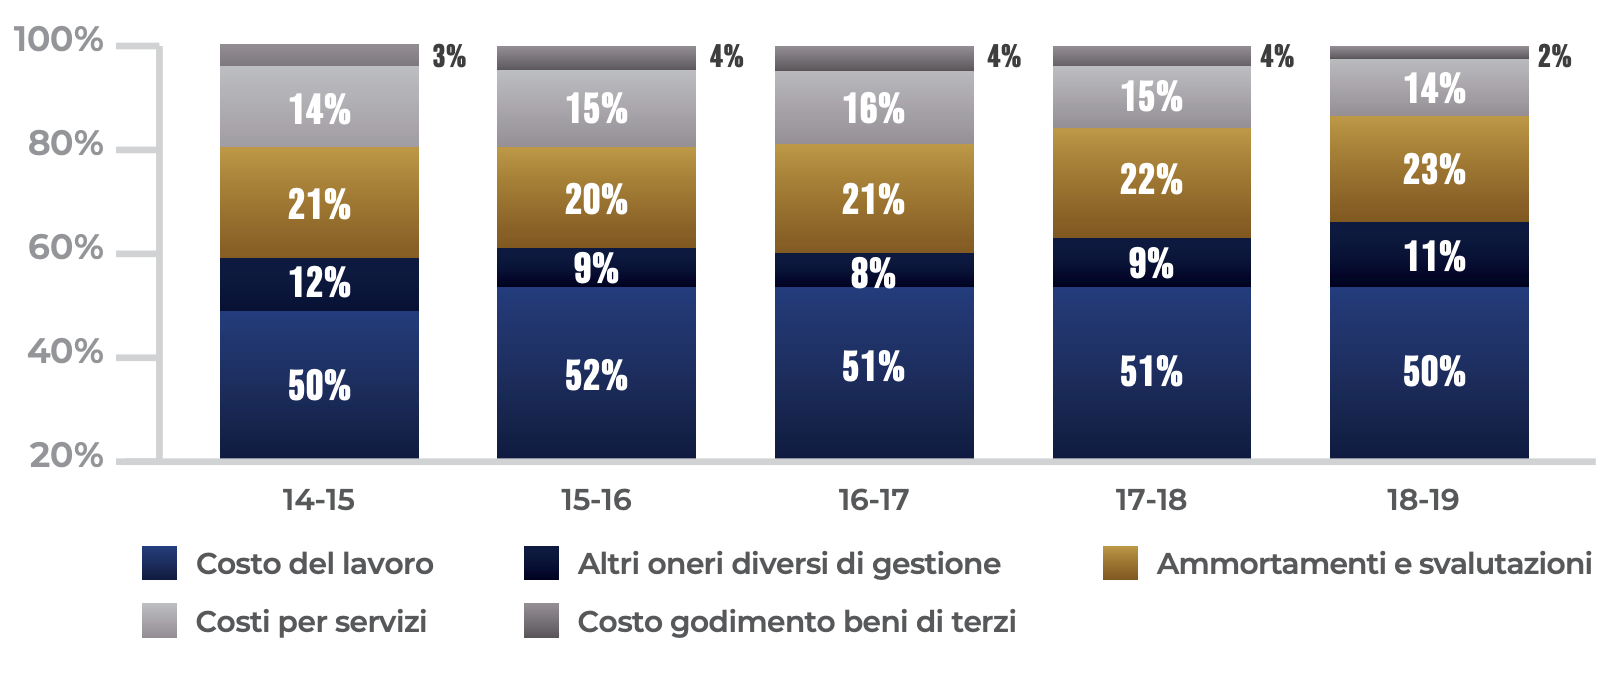
\includegraphics[width=.55\textwidth]{img/wage_serieA.png} \label{figA}} \quad
    \subfloat[][Confronto stipendi Serie A 17/18 e 18/19]
    {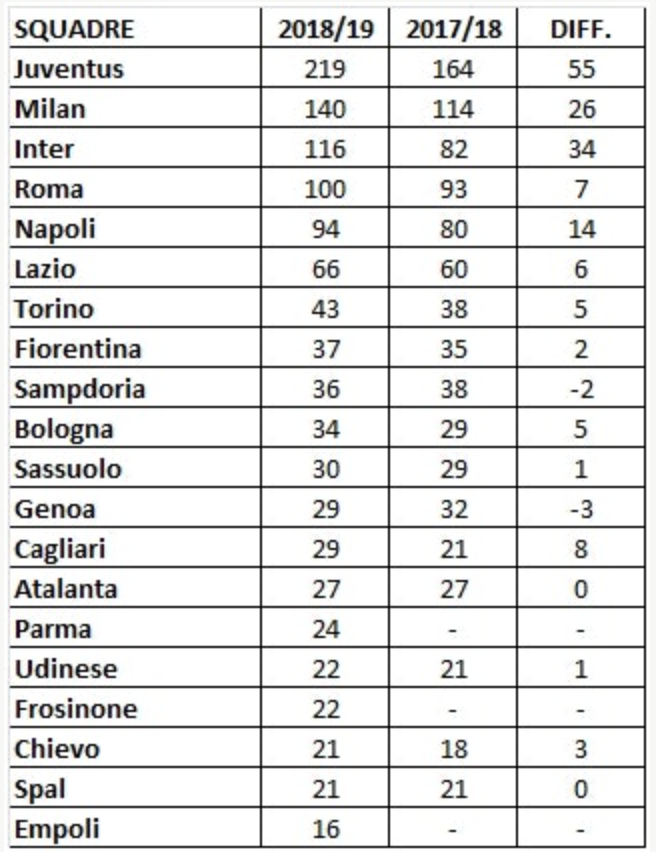
\includegraphics[width=.25\textwidth]{img/diff_wage_serieA.png} \label{figB}}
    \caption{Situazione \emph{Costo del Lavoro} all'interno del calcio italiano}
    \label{wage_serieA}  
\end{figure}
Il problema di questo momento di respiro \'e che si tratta di un qualcosa a breve termine che scomparir\'a quando Cristiano Ronaldo e la 
sua immagine non saranno pi\'u legati alla Serie A.\newpage
Per quanto riguarda invece la \textbf{Francia}, l'organizzazione che si occupa del monitoraggio e la supervisione dei conti 
delle società calcistiche è la DNCG\footnote{Direction Nationale du Contrôle de Gestion}. Essa 
pubblica ogni stagione un report riassuntivo per quanto riguarda la Ligue 1 e la Ligue 2 (i primi due campionati francesi) ed una
relazione relativa ad ogni singolo club dei due campionati. Tutti i dati di seguito riportati sono stati reperiti dai singoli
report annuali pubblicati \footnote{https://www.lfp.fr/dncg/rapports} \newline
Al termine della stagione 2018/2019 il \textbf{Risultato Netto "consolidato"} ammontava a -160mln€, in miglioramento per\'o del 9\% rispetto 
all'anno prima (-176). Questo risultato, come indicato prima, \'e il risultato della sottrazione tra ricevi e costi d'esercizio
dei due campionati. Andando ad analizzare nello specifico i due risultati \'e possibile notare come la Ligue 1 abbia 
osservato un incremento del 20\% del Risultato Netto rispetto alla stagione precedente ma la Ligue 2 ha 
dovuto affrontare un calo del 90\% del Net Profit, andando quindi completamente ad annullare il risultato del 
campionato superiore. 
La perdita registrata nella stagione 18/19 \'e la seconda in termini di importanza a partire dalla stagione 2013/2014 e
il motivo principale che spiega questa discesa cos\'i decisa, \'e da attribuirsi ad un aumento delle entrate (\emph{Income}),
con un valore che passa da 304 mln€ nel 17/18 a 316 mln€ nel 18/19, che per\'o non riesce a controllare l'aumento pi\'u considerevole
delle spese (\emph{Expenses}), sopratutto nella sezione dedicata alle spese proprie dei club: stipendi di giocatori e commissioni degli agenti; 
oltre alla sezione "Altre Spese" (\emph{Other Expenses}), queste due voci aumentano rispettivamente di 5 e 9 mln€.\newline
Il secondo indicatore che viene preso in considerazione \'e chiamato \textbf{Payroll}, termine indicante la somma dei vari stipendi
dei dipendenti di un club. Nonostante un Payroll, almeno per quanto riguarda le squadre qualificate per la UCL \footnote{Uefa Champions League}, in linea con gli
altri campionati (147 mln€ nella Premier League inglese \footnote{Calcolo personale utilizzando i dati da https://www.spotrac.com/epl/payroll/})
i risultati ottenuti nelle competizioni internazionali non sono state all'altezza: nella stagione 2018/2019 sono presenti 3 squadre 
all'interno della fase a gironi della massima competizione europea: Monaco, Paris Saint Germain e Olympique Lione. La prima si 
posizione ultima nel gruppo A, la seconda (da cui gli esperti e i sostenitori si aspettano grandi risultati, visti i milioni di euro 
spesi ogni anno) viene eliminata agli ottavi di finale e infine la terza viene anch'essa eliminata agli ottavi di finale. Questo scenario
si ripete mediamente ogni anno, mentre, se si vuole trovare una squadra francese vincitrice dobbiamo tornare indietro alla stagione 1992/1993
con l'Olympique Marsiglia.\newline
Ripartendo dall'ultimo indicatore analizzato e collegandolo al primo \'e possibile constatare come i grandi investimenti spesso non portano 
al successo assicurato e quindi ad un ritorno concreto. Queste grosse somme che escono dalle casse dei club che per\'o
non vedono un ritorno portano un danno a tutto il campionato, perch\'e da un lato viene aumentato il gap tecnico tra le diverse squadre dello
stesso campionato mentre dall'altro, in campo internazionale, non si ottengono risultati non ricevendo quindi premi da sponsor e organizzatori.
Tutto questo circolarit\'a non fa' altro che danneggiare il sistema calcio francese perch\'e si fa perdere valore e quindi appeal, sia 
visivo che economico, al campionato locale e si "danneggia" l'immagine europea dei club francesi, considerati incapaci, nonostante le somme spese,
di ottenere risultati.
\end{interlinea}

\end{document}

